\documentclass[tikz,border=5pt]{standalone}
\usepackage[T1]{fontenc}
\usepackage{lmodern,amsmath,amssymb}
\usetikzlibrary{arrows.meta,calc,positioning,fit,backgrounds,shapes.geometric,matrix,decorations.pathreplacing,patterns}
\definecolor{ink}{gray}{0.08}
\definecolor{wash}{gray}{0.965}
\definecolor{soft}{gray}{0.45}
\tikzset{box/.style={draw=ink,line width=.65pt,fill=white,align=center,inner sep=4pt,outer sep=0pt,font=\small},flow/.style={draw=ink,line width=.65pt,-{Latex[length=1.8mm,width=1.3mm]},rounded corners=2pt},annotation/.style={font=\scriptsize,text=soft,align=center},groupbox/.style={draw=soft,dashed,line width=.45pt,fill=wash}}
\begin{document}
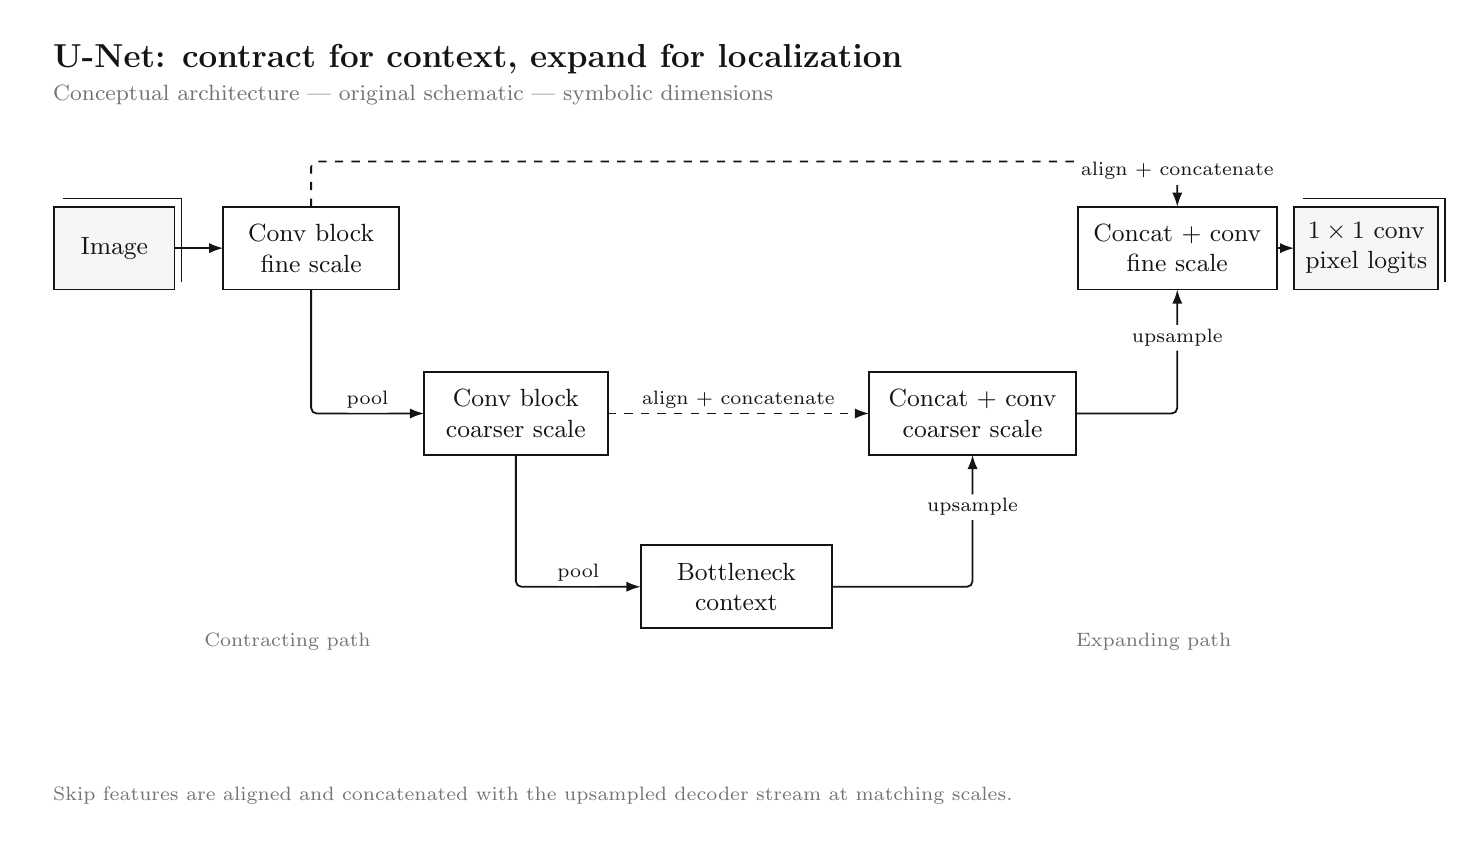
\begin{tikzpicture}[x=1cm,y=-1cm,font=\rmfamily,text=ink]

\path[use as bounding box] (0,0) rectangle (18,10);
\node[anchor=west,font=\large\bfseries] at (.2,.4) {U-Net: contract for context, expand for localization};
\node[anchor=west,font=\footnotesize,text=soft] at (.2,.85) {Conceptual architecture | original schematic | symbolic dimensions};
\begin{pgfonlayer}{background}
\end{pgfonlayer}
\node[box,fill=wash,minimum width=1.5cm,minimum height=1.05cm,text width=1.25cm] (x) at (1.1,2.8) {Image};
\draw[ink,line width=.4pt] (0.45000000000000007,2.175) -- (1.9500000000000002,2.175) -- (1.9500000000000002,3.2249999999999996);
\node[box,minimum width=2.2cm,minimum height=1.05cm,text width=1.9500000000000002cm] (e1) at (3.6,2.8) {Conv block\\fine scale};
\node[box,minimum width=2.3cm,minimum height=1.05cm,text width=2.05cm] (e2) at (6.2,4.9) {Conv block\\coarser scale};
\node[box,minimum width=2.4cm,minimum height=1.05cm,text width=2.15cm] (b) at (9.0,7.1) {Bottleneck\\context};
\node[box,minimum width=2.6cm,minimum height=1.05cm,text width=2.35cm] (d2) at (12.0,4.9) {Concat + conv\\coarser scale};
\node[box,minimum width=2.5cm,minimum height=1.05cm,text width=2.25cm] (d1) at (14.6,2.8) {Concat + conv\\fine scale};
\node[box,fill=wash,minimum width=1.8cm,minimum height=1.05cm,text width=1.55cm] (y) at (17.0,2.8) {$1\times1$ conv\\pixel logits};
\draw[ink,line width=.4pt] (16.200000000000003,2.175) -- (18.0,2.175) -- (18.0,3.2249999999999996);
\begin{pgfonlayer}{background}
\draw[flow] (x.east) -- (e1.west);
\draw[flow] (e1.south) -- (3.6,4.9) -- (e2.west) node[midway,above,fill=white,inner sep=1.5pt,font=\scriptsize] {pool};
\draw[flow] (e2.south) -- (6.2,7.1) -- (b.west) node[midway,above,fill=white,inner sep=1.5pt,font=\scriptsize] {pool};
\draw[flow] (b.east) -- (12,7.1) -- (d2.south) node[midway,above,fill=white,inner sep=1.5pt,font=\scriptsize] {upsample};
\draw[flow] (d2.east) -- (14.6,4.9) -- (d1.south) node[midway,above,fill=white,inner sep=1.5pt,font=\scriptsize] {upsample};
\draw[flow,dashed] (e2.east) -- (d2.west) node[midway,above,fill=white,inner sep=1.5pt,font=\scriptsize] {align + concatenate};
\draw[flow,dashed] (e1.north) -- (3.6,1.7) -- (14.6,1.7) -- (d1.north) node[midway,above,fill=white,inner sep=1.5pt,font=\scriptsize] {align + concatenate};
\draw[flow] (d1.east) -- (y.west);
\end{pgfonlayer}
\node[annotation,text width=4cm] at (3.3,7.8) {Contracting path};
\node[annotation,text width=4cm] at (14.3,7.8) {Expanding path};
\node[anchor=west,align=left,font=\scriptsize,text=soft,text width=17.6cm] at (.2,9.75) {Skip features are aligned and concatenated with the upsampled decoder stream at matching scales.};
\end{tikzpicture}
\end{document}
